\section{Hjertet}\label{Hjerte}


Hjertet er essentielt for kroppens funktion. Dette tydeliggør sig f.eks. ved at hvis hjertet holder op med at slå, vil den pågældende person miste bevidstheden allerede efter 5-10 sekunder. 

\subsection{Overordnet anatomi \& fysiologi}\label{Hjerte_ana_fys}

Hos et voksent menneske, er hjertet omtrent lige så stort som en knyttet hånd, og vejer ca 300-350 gram for mænd, hvorimod kvinders hjerte har en vægt på omtrent 250-300 gram. Hjertet er placeret bag sternum i thoraxhulen som ses på figur \ref{fig:hjerte_placering}. %, for midtlinjen

\begin{figure}[H] % Example of including images
\begin{center}
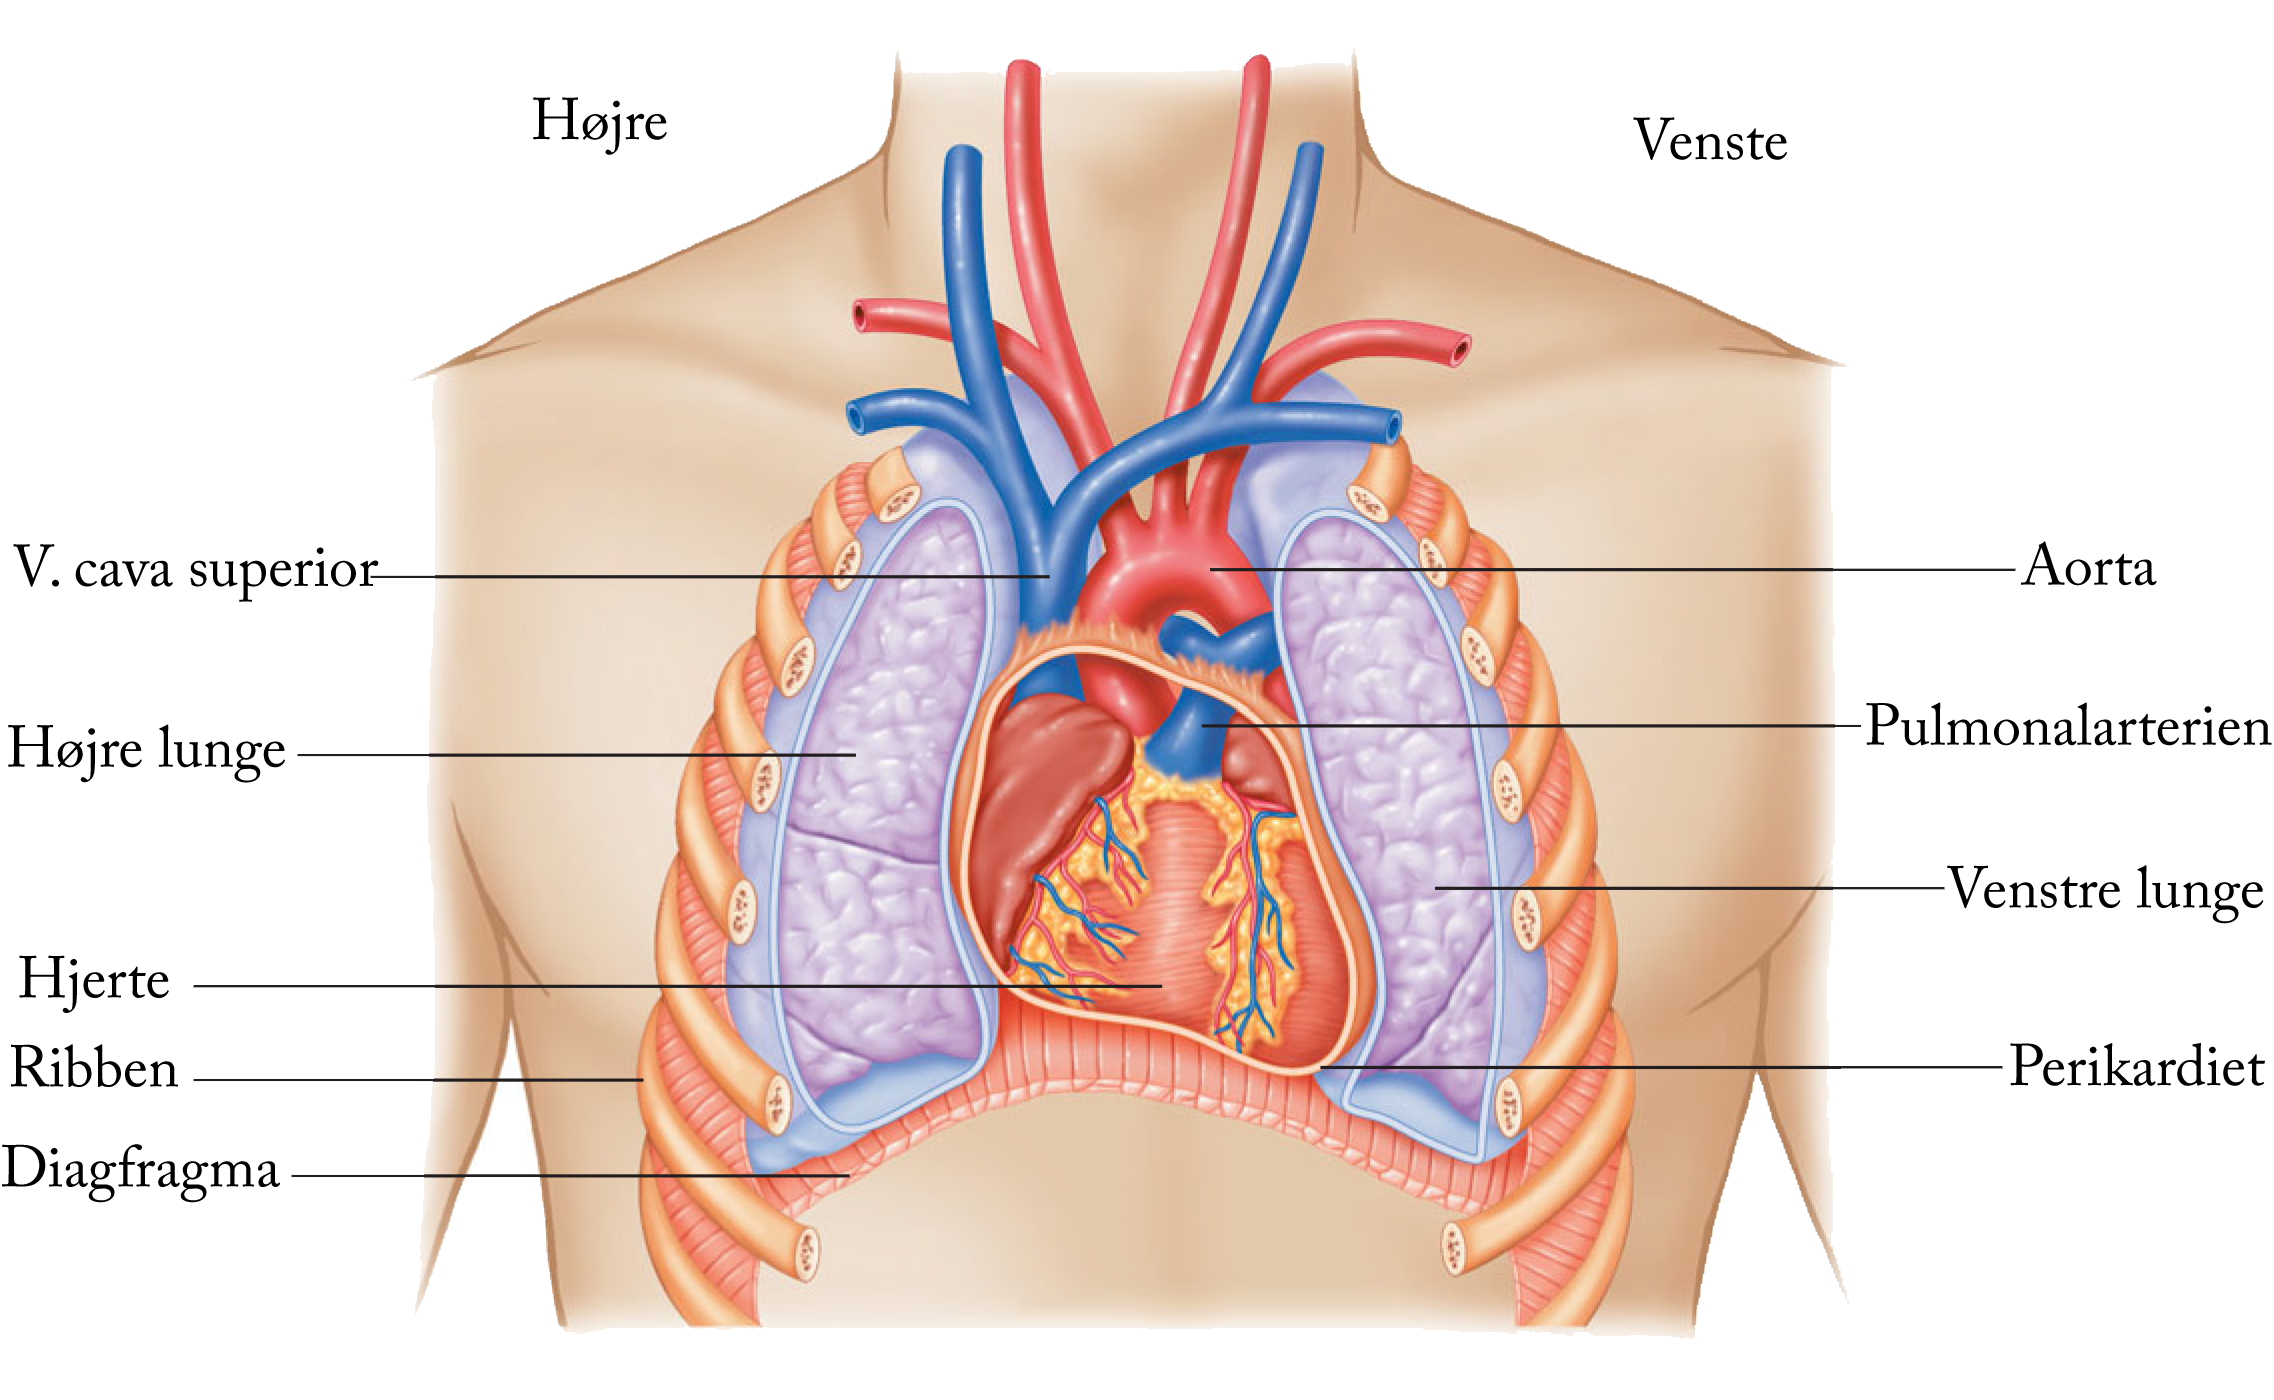
\includegraphics[width=1\textwidth]{figures/thorax}
\end{center}
\caption{Illustration af hjertets placering i thoraxhulen. \cite{cindy}}
\label{fig:hjerte_placering}
\end{figure}

Hjertet er omgivet af perikardiet, som består af kollagene fibre. Laget er med til at stabilisere hjertet og dets tilhørende blodkar i mediastinum, og desuden er denne med til at smøre hjertet.


Hjertet fungerer som en pumpe, der pumper blod rundt i hele kroppen vha. trykforskelle med et interval bestemt af hjertets elektriske signal. Disse trykforskelle opstår fordi hjertet er et hult muskelorgan med fire kamre; højre og venstre atrium, og højre og venstre ventrikel samt en række klapper til at holde blodet inde ller ude. Som ses på figur \ref{fig:hjerte_overordnet}

\begin{figure}[H] % Example of including images
\begin{center}
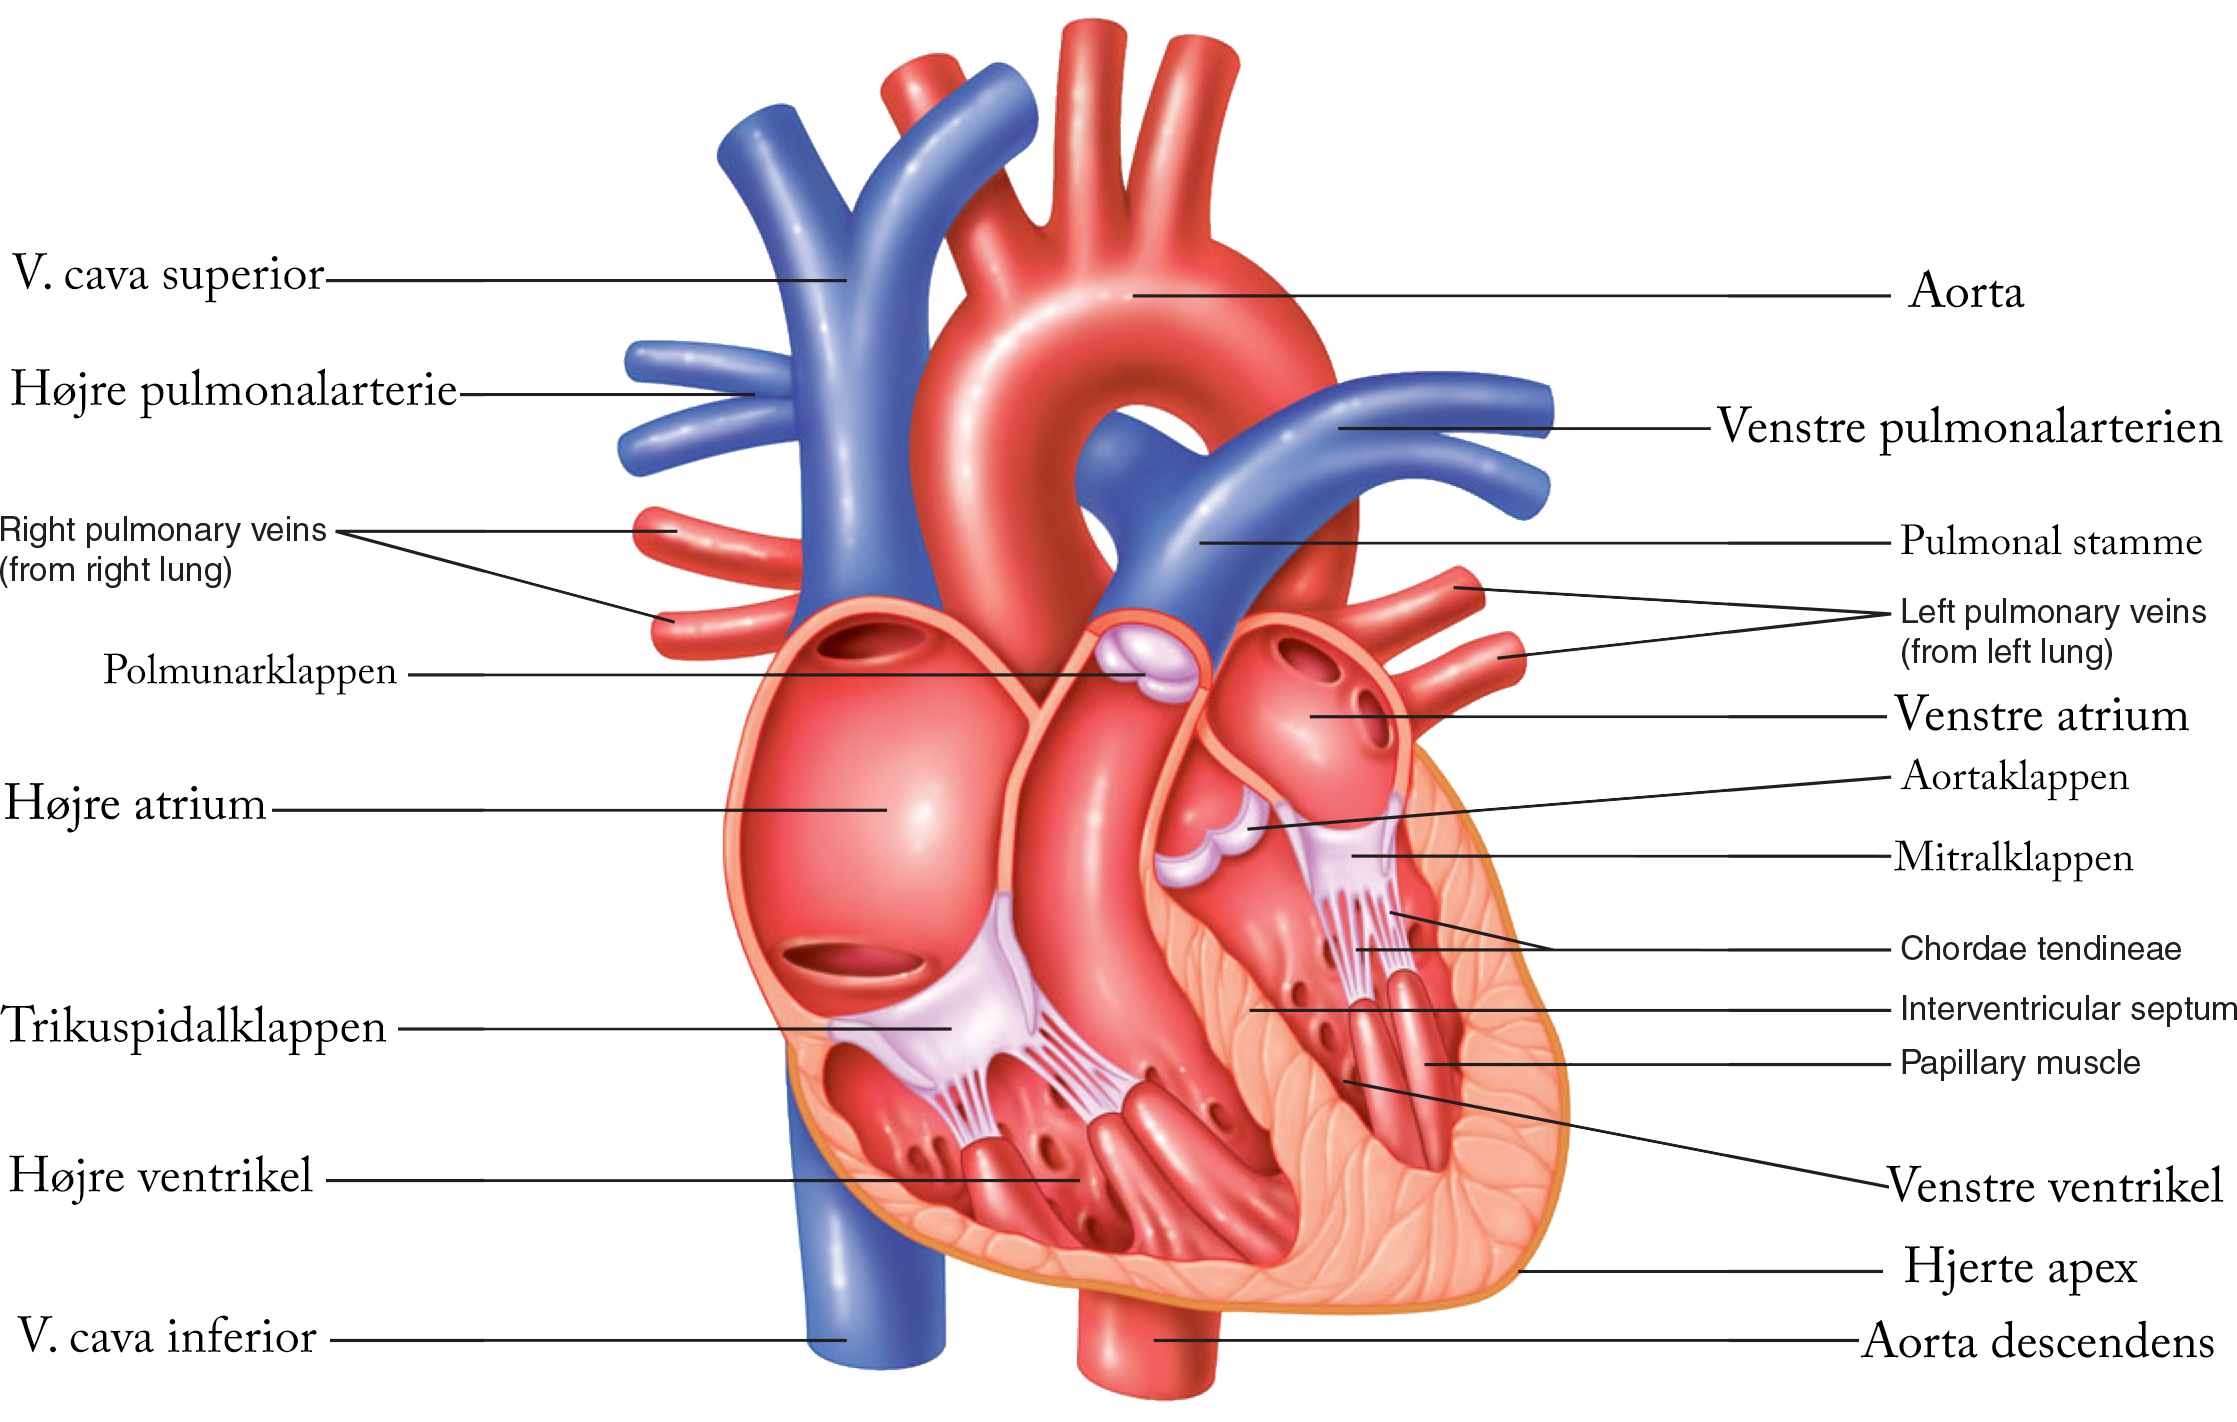
\includegraphics[width=0.5\textwidth]{figures/hjertet_overordnet}
\end{center}
\caption{Illustration af hjertets overordnet anatomiske opbygning \cite{Guyton2006}}
\label{fig:hjerte_overordnet}
\end{figure}


Hjertevæggen består af tre lag; endokardiet, myokardiet og epikardiet. Myokardiet er det midterste lag i hjertevæggen og dette lag består af hjertemuskelceller som udgør hjertets muskulatur \cite{gronanatomi}. Hjertevæv består hovedsagligt af disse celler, og disse er også hovedansvarlige for at udføre hjertets gentagne kontraktioner, hvor hjertevæggen bevæger sig indad \cite{cindy}. 
Hjertemuskelceller diffenrecierer sig fra skeletmuskelceller bl.a. ved at de er forgrenede, deres størrelse er mindre, de besidder kun en enkelt cellekerne per celle og imellem cellerne er indskudsskiver der kan fører aktionpotentialerne videre \cite{martini}.




\subsubsection{Hjertets blodforsyning}
Ca. 4\% af hjertets minutvolumen går igennem koronararteriene som forsyner hjertet, på trods af at hjertet kun udgør ca. 0,4\% af den samlede legemsvægt \cite{gronanatomi}. Hjertemuskelceller stiller høje krav til tilførelse af ilt og næringstoffer ifht. til de fleste andre væv i kroppen. Hjertet er nemlig ikke i stand til, på samme måde som andre væv, at udføre anaerob metabolisme, og faktisk vil hjertet bruge mere end 70 \% af den ilt der tilføres til hjertet. Under anstrengelse kan blodgennemstrømningen i hjertet stige til det 9 dobbelte ifht. når kroppen befinder sig i afslapning \cite{martini}. Koronararterierne afgår fra aorta tæt på aortaklappen. A. coronaria dextra forsyner hovedsageligt højre del af hjertet med blod, og a. coronaria sinistra forsyner hovedparten af den venstre side af hjertet. Ramus interventricularis anterior som er beliggende på den anterior del af hjertet forsyner de forreste dele af ventrikelskillevæggen og de dele der støder op til denne \cite{gronanatomi}.


\subsection{Hjertets cyklus}
Blodet i hjertet pumpes rundt, ved at kontraktioner. Kontraktionerne skaber forskellige tryk i hjertekamrene. Atrierne kontraheres samtidig, og ligeledes kontraheres ventriklerne samtidig. Dog vil trykket i højre halvdel kun opnå ca. 20 \% af det maksimale tryk der opnåes i venstre ventrikel. Dette skyldes at den højre halvdel kun skal pumpe blod ud til lungerne, hvorimod at den venstre side har til opgave at pumpe blod rundt i hele kroppen. Generelt kan hjertets cyklus opdeles i 2 dele; systole (ventriklerne er kontraherede)  og diastole (ventriklerne er afslappede). En mere detaljeret gennemgang fra et mekanisk perspektiv er som følgende: \cite{gronanatomi}.


\begin{itemize}
\item Ventrikler er afslappede. Når trykket bliver lavere end atrierne åbnes AV-klapperne. Dette resulterer i at ventriklerne fyldes passivt med blod. Blodet kommer ind i højre atrium via v. cava superior og inferior.
\item Atrierne kontraherer og derved fyldes ventriklerne yderligere.
\item Ventriklerne påbegynder kontraktion. Dette resulterer i at AV-klapperne lukkes.
\item Ventriklernes tryk overstiger trykket i arterierne. Dette resulterer i at semilunærklapperne åbnes og blodet strømmer ud i aorta og pulmonalarterien.
\item Ventriklerne afslappes, og trykket bliver lavere end arteriernes. Dette betyder at semilunærklapperne lukkes. Når ventrikeltrykket bliver lavere end trykket i atrierne åbnes AV-klapperne og dermed starter cyklussen påny.
\end{itemize}


\begin{figure}[H] % Example of including images
\begin{center}
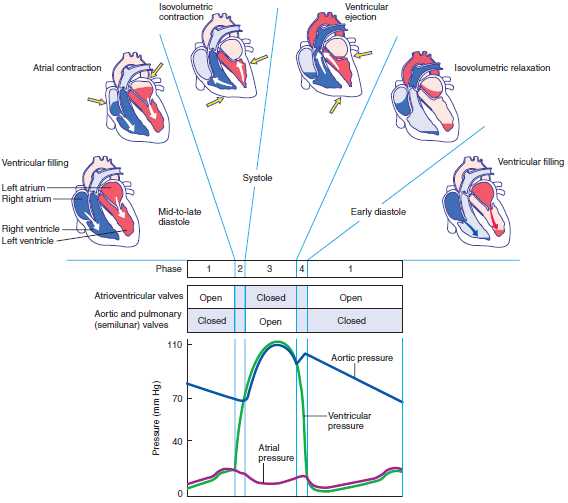
\includegraphics[width=1\textwidth]{figures/cyklus}
\end{center}
\caption{Illustration af hjertets cyklus\cite{cindy}}
\label{fig:hjerte_cyklus}
\end{figure}

\subsubsection{Hjertets klapper}
For at blodet skal strømme i den rigtige retning, har hjertet fire klapper; atrioventrikulærklapperne, som består af trikuspidalklappen, (mellem højre atrium og ventrikel), mitralklappen (mellem venstre atrium og ventrikel) og semilunærklapperne aorta- samt polmunarklappen. Semilunærklapperne funktion er at forhindre reflux af blodet til henholdsvis venstre og højre ventrikel som ilusteres på figur \ref{fig:hjerte_klap}.  \cite{gronanatomi}  

\begin{itemize} 
	\item Atrioventrikulærklapperne
		\begin{itemize} 

			\item Trikuspidalklappen, (mellem højre atrium og ventrikel)
			\item Mitralklappen (mellem venstre atrium og ventrikel)

		\end{itemize} 


	\item Semilunærklapperne

		\begin{itemize} 

			\item Aortaklappen
			\item Polmunarklappen

		\end{itemize} 		
\end{itemize} 


\begin{figure}[H] % Example of including images
\begin{center}
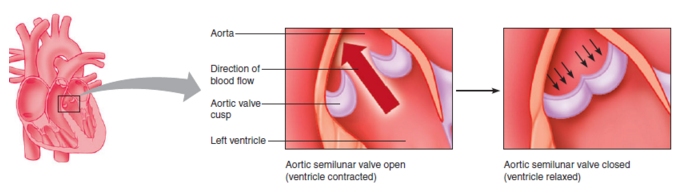
\includegraphics[width=1\textwidth]{figures/cusp}
\end{center}
\caption{Illustration af klappernes funktion med eksempel af aorta klappen. \cite{cindy}}
\label{fig:hjerte_klap}
\end{figure}

\subsection{Hjertets elektriske ledningssystem}\label{Hjertets_elektriske_ledningssystem}
Hjertets rytmiske kontraktioner som får blodet til at pumpe rundt udføres vha. hjertets elektriske ledningssystem. Ved skade på det elektriske system kan det resultere i en unormal hjerterytme eller abnormale kontraktioner af hjertet der medfører en svækkelse af hjertes pumpefunktion \cite{guyton}. Hjertemuskulaturen har den specielle evne, at den kan kontrahere sig selv uden at modtage et nervesignal \cite{gronanatomi}. Hjertet er dog også forsynet med sympatiske og parasympatiske nerver, og disse er med til at regulere hjerterytmen \cite{cindy}. 
Hjertets ledningssystem består SA-knuden, Det his'ske bundt, grenbundterne og purkinjefibrene \ref{fig:hjerte_elektriske}.
Aktionspotentialer der får hjertet til spontant at kontrahere, og dermed bestemme hvilken frekvens hjertet slår med, initieres i sinusknuden (SA-knuden), og derfor bærer cellerne i SA-knuden også navnet "pacemaker" celler.
Sinusknuden er beliggende i den øverste del af højre atrium og cellerne i SA-knuden vil typisk fyre 60 til 100 gange i minuttet, men dette er stærkt afhængigt af det autonome nervesystems aktivitet, samt kroppens behov for at øge hjertets
minutvolumen \cite{ekgbook}.

\begin{figure}[H] % Example of including images
\begin{center}
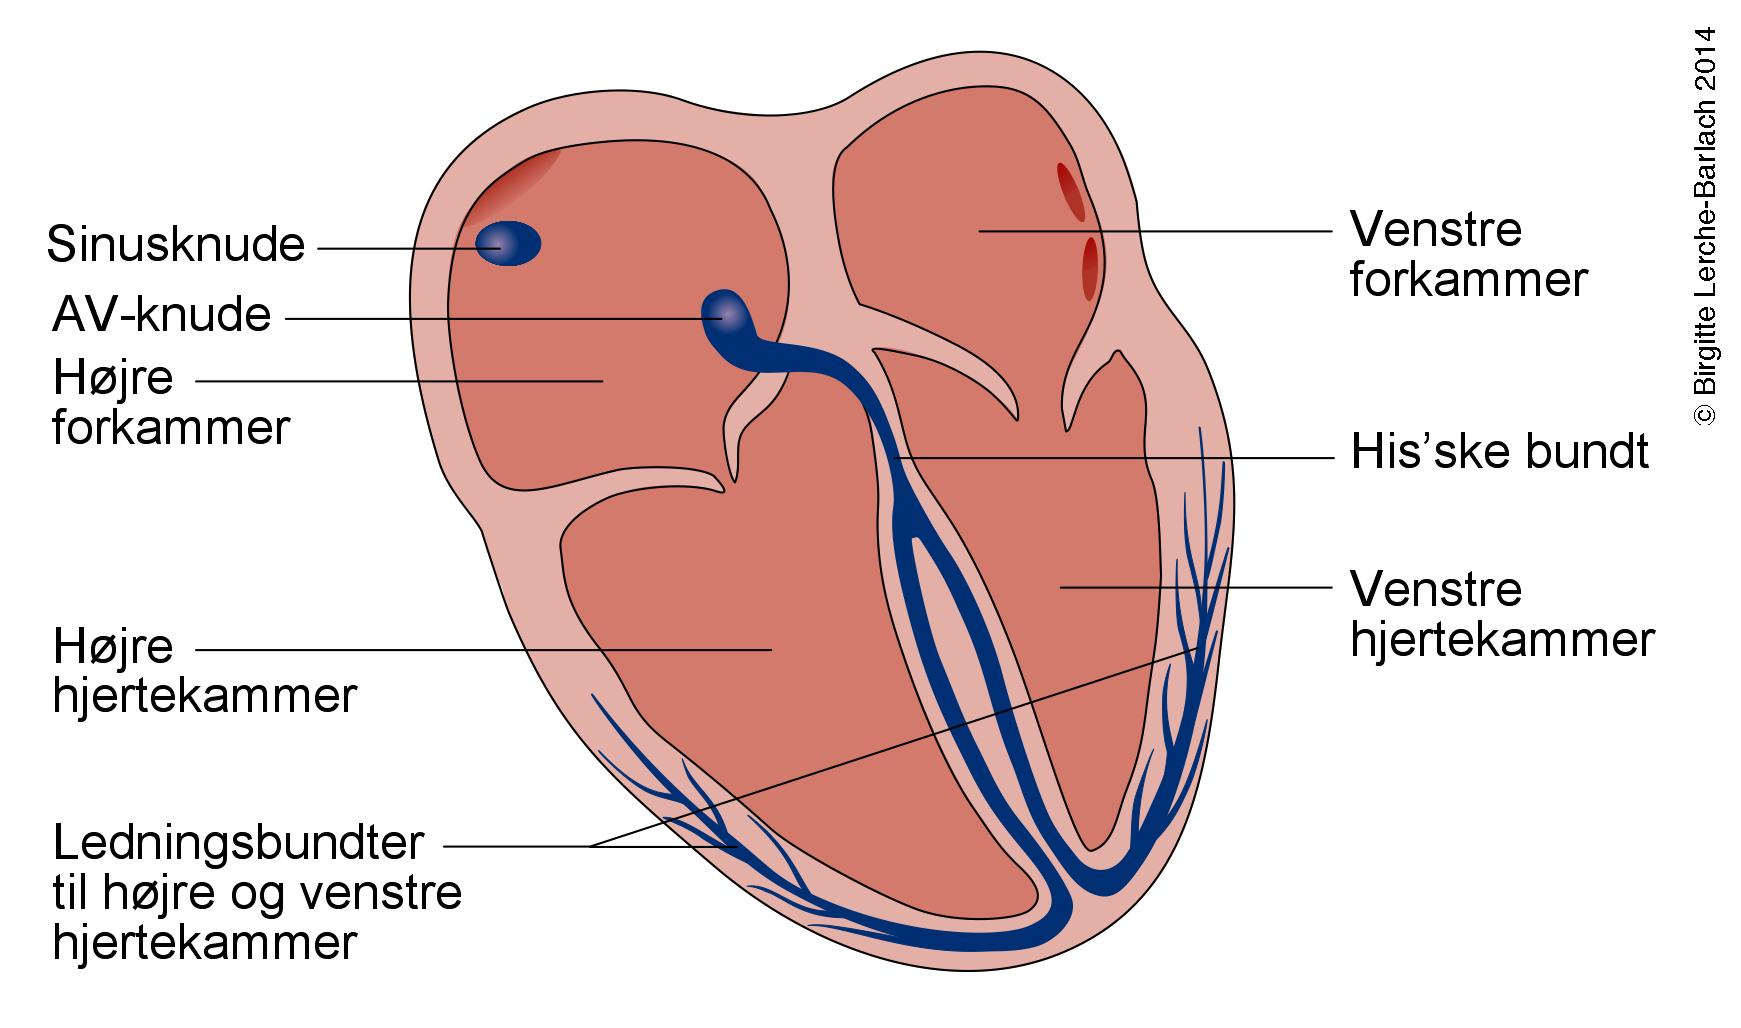
\includegraphics[width=1\textwidth]{figures/hjerte_elektrisk}
\end{center}
\caption{Illustration af hjertets eleketriske system.\cite{elektriske}}
\label{fig:hjerte_elektriske}
\end{figure}

SA-knudens signal føres til forskellige områder af hjerter på to måder. Enten ved at hjertemuskelcellerne fører signalet videre til en anden hjertemuskelcelle via gap junctions (åbne celleforbindelser), eller fra celle til celle i hjertets specielle ledningssystem, som består af specialiserede hjertemuskelceller, og dette udføres også vha. af gap-junctions \cite{gronanatomi}. 
Disse gap-junctions muliggør en hurtig diffussion af ioner \cite{guyton}.
AV-knudens primære opgave er at  forsinke det elektriske signal. Ved et normalt fungerende hjerte vil atrierne kontrahere ca. en en sjettedel af sekund før ventriklerne, og dette er fordi ventriklerne skal have mulighed for at forsynes med en tilstrækkelig mængde blod\cite{guyton}.
Det hisske bundt der fører signalet gennem anulus fibrosus som er den eneste elektriske forbindelse mellem atrierne og ventriklerne, derefter går his'ske bundt over i grenbundterne der fører signalet videre. Purkinjefibrene leverer signalet til det ventrikulære myokaridum og disse fibre har den egenskab at de kan lede de elektriske signalet hurtigt. Indenfor 75 ms af ventriklernes depolariseret\cite{gronanatomi}. Hele depolariseringsprocessen strækker sig ca. over 225 ms.



